\chapter{Introduction}
\label{Introduction}

\section{Context}

Arguably, humans rely on their sense of sight more than any other sense in understanding the world around them. Finding our way in a busy street, locating a book on a shelf in a library and interacting with hundreds of objects in our everyday life are some of examples that require extensive use of visual cues. We can not only recognise objects and locations, but also create a 3D structure of the scene in our mind. Even by looking at a single image, we can answer complex questions about position, orientation, and relation of objects. 

As technologies such as augmented reality, self-driving cars, drones, and robotics in general, progress towards finding more use cases in our every day lives, the need for better scene understanding in real 3D space increases. By advent of intelligent personal assistant softwares and smarter applications, providing more useful features and better user experience depends on understanding the real world that users live in it.

Scene understanding is one of the most fundamental problems in computer vision. It is very challenging to solve this problem by only using 2D visual data captured by ordinary cameras. Thus, hardware manufacturers have tried to make this task easier by providing more information about the 3D space; using a variety of camera arrays, structured light 3D scanners, and time-of-flight (ToF) sensors. 3D vision systems use these sensors to measure, map, locate, and reconstruct the three dimensional structure of the environment for visual perception tasks.  

Data provided by these sensors, plays a crucial role in many currently popular products in fields of augmented reality, robotics, biometric facial recognition, and gesture detection (e.g. Microsoft Kinect, Apple FaceID, and Tesla Autopilot). But in many applications, access to these sensors is not simply possible. For example, the vast amount of images and videos currently available on the internet, provide no extra 3D information about their content. On the other hands, in comparison to humans, software systems are unable to fully exploit the visual information that 2D images contain. Therefore, there is still a strong need for developing more advanced scene understanding and reconstruction systems that are based on 2D input data.      

Estimating the orientation of surfaces in an image, is an important step in reconstructing a 3D model of the scene. Recently, the surface normal estimation from monocular RGB images, has been an active area of research in computer vision. Tackling this problem is the main topic of this M.Sc. project. 

\pagebreak

\section{Problem Statement} \label{problemstatement}

Before any further discussion, a precise definition of the problem is needed. In this project, the problem of pixel-wise surface normal estimation from monocular RGB images of the indoor scenes is addressed. 

The RGB images are captured from indoor environments with realistic scene layout such as bedrooms, living rooms, kitchens, and offices. Figure \ref{fig:scene} illustrates a typical scene layout and viewpoint. 

\begin{figure}[h]
    \centering
    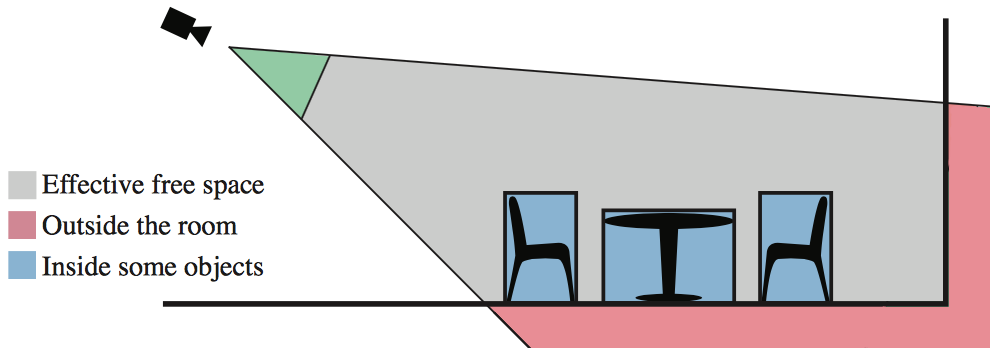
\includegraphics[scale=0.35]{Scene}
    \caption{Schematic view of a scene, adapted from \cite[p.~5]{sun}}
    \label{fig:scene}
\end{figure}

Given an RGB image as input, the estimated surface normal map is expected as output. Samples of RGB images and the corresponding normal maps are illustrated in figure \ref{fig:gt}. 

\begin{figure}[h]
    \centering
    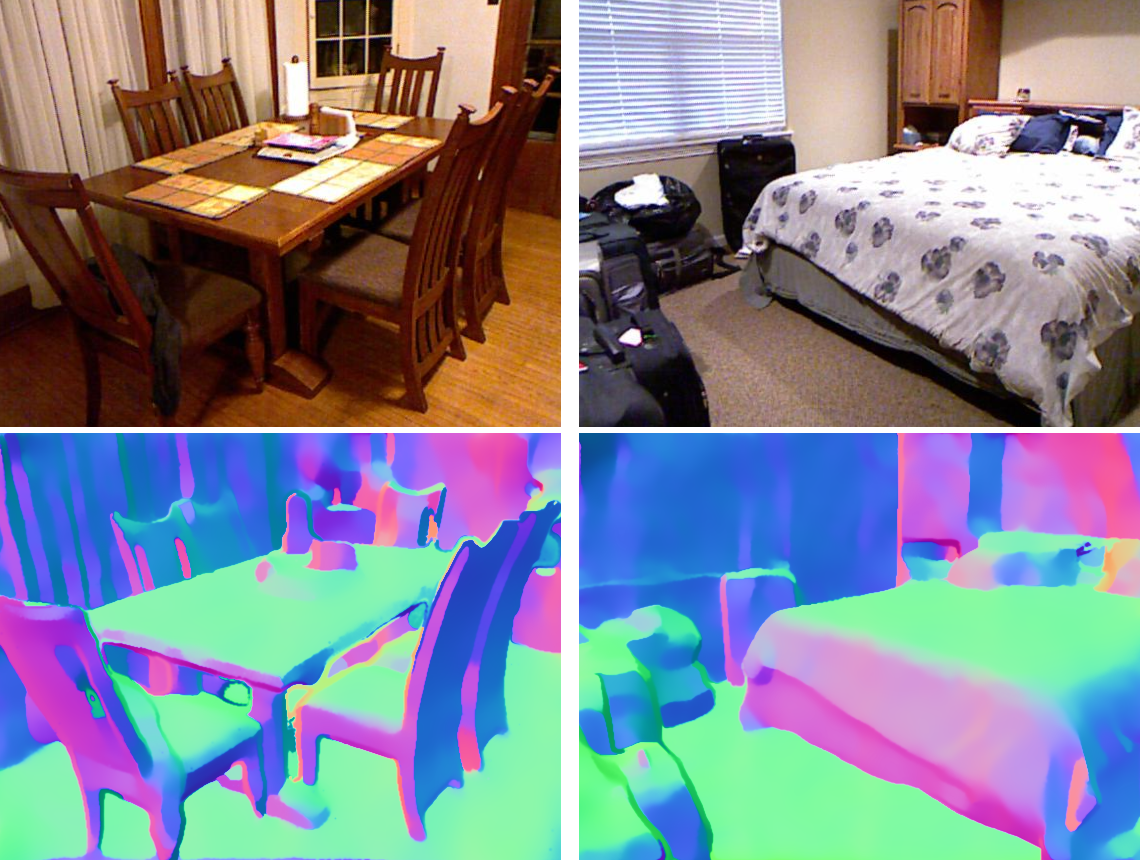
\includegraphics[scale=0.3]{GT}
    \caption{Top: RGB images of indoor scenes, Bottom: corresponding surface normal maps \\
    Normal legend: {\color{blue} $blue\rightarrow X (horizontal)$}; {\color{green} $green\rightarrow Y (vertical)$}; {\color{red} $red\rightarrow Z (perpendicular\ to\ image)$}.}
    \label{fig:gt}
\end{figure}


\section{Proposed Solution}

In last few years, deep learning has made major breakthroughs in field of computer vision.  Deep neural networks (DNNs) have achieved impressive performance in challenging tasks such as image classification, semantic segmentation, and image compression. DNNs have started to even exceed human performance in tasks such as image classification \cite{humanvsdnn}. Therefore it is not surprising that current state of the art solutions for the task of surface normal estimation are all based on deep learning. 

Based on the promising achievements of deep neural networks, and the huge gap between the results yielded by using these networks in comparison to traditional methods in similar problems, a solution based on DNNs was chosen as the preferred approach for this project. At first, a baseline network architecture was implemented and after training the model, the estimated surface normal maps were evaluated.  Afterwards, based on the insights gained from the literature review and analysis of the state of the art methods, different modifications to the baseline model were investigated. In particular, improvements over baseline results were explored in respect to two aspects: network architectures, and the quality of data set.   

\section{Project Aim}

This project explored a deep learning approach for the task of surface normal estimation. The data needed for training and evaluation of the system, was acquired by using publicly available data sets. Different network architectures were implemented and finally, well-established evaluation metrics were used to compare the results with the previous research in this field. 

\subsection{Objectives}

\begin{itemize}
    \item Data set and ground truth acquisition
    \item Analysing the state-of-the-art methods
    \item Proposing a new method or improvements over current methods and
implementing it
    \item Evaluating the method and comparing with other methods
\end{itemize}

\subsection{Deliverables}

\begin{itemize}
    \item Data set
    \item Analysis of the state-of-the-art methods
    \item Source code and algorithms
    \item Evaluation results
\end{itemize}

\section{Planning and Project Management}

Before starting the work on this project, a period of two months was spent on background study and literature review. During this period, works relevant to the subject of this project were identified, and the theoretical aspects of the solutions discussed in existing research, were studied. A better understanding of the problem, and a proposed solution were the outcomes of this process. 

\subsection{Initial Plan}
To guide the project execution, an initial plan was devised and the project was broken down to four main tasks: 

\begin{itemize}
    \item \emph{Data Acquisition and Preparation}: preparing the data sets required for training and evaluation of the system
    \item \emph{Analysis of Related Work}: studying the source codes released by relevant works and reproducing their results
    \item \emph{Implementation and Evaluation}: implementing the system and evaluating the results
    \item \emph{Report Writing}: writing the project report
\end{itemize}

Based on these tasks, an initial project schedule for a period of three months was created (figure \ref{fig:initialplan}). 

\begin{figure}
    \centering
    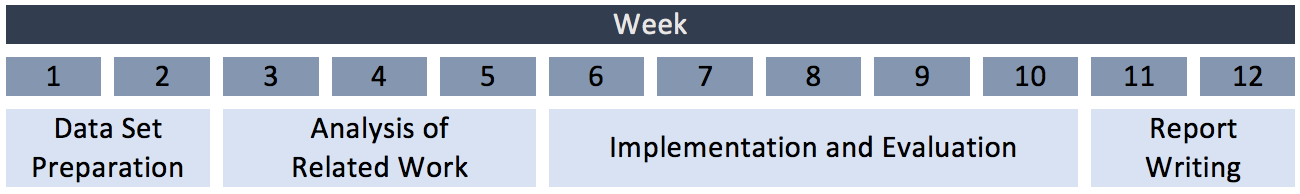
\includegraphics[width=\textwidth]{InitialPlan}
    \caption{Initial project plan}
    \label{fig:initialplan}
\end{figure}

\subsection{Revised Plan}
In reality, the time that was spent on different tasks was different with what initially was planned. Because of difficulties in data set preparation task, one more week than expected was spent on this task. Also, analysis of related work took one week less than expected. After two months, in a progress meeting with supervisor and assessor of the project, the project plan was reconsidered. 

\begin{figure}[h]
    \centering
    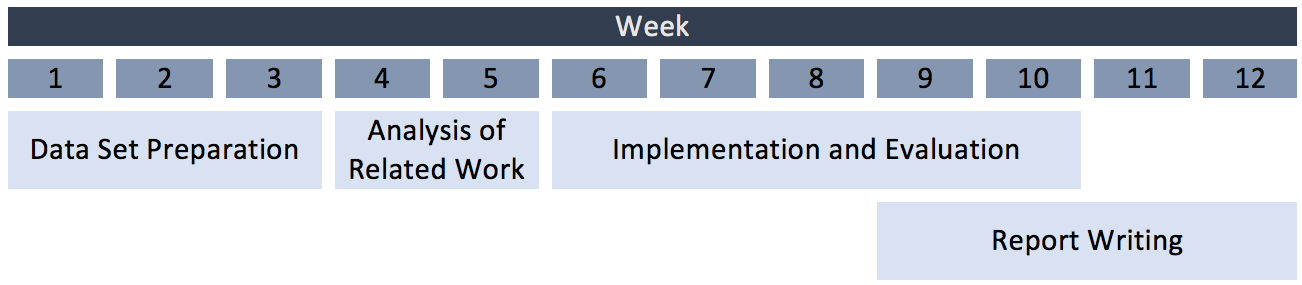
\includegraphics[width=\textwidth]{RevisedPlan}
    \caption{Revised project plan}
    \label{fig:revisedplan}
\end{figure}

Figure \ref{fig:revisedplan} illustrates the revised project plan. Based on the provided suggestions, the time considered for writing the project report was extended to four weeks, starting in parallel to last weeks of project implementation and evaluation. 

\subsection{Methodology}
The methodology used for this project was mainly based on performing a series of experiments to gradually design better network architectures. The implementation and evaluation task was conducted based on the workflow illustrated in figure \ref{fig:workflow}. After preparing the data sets, for each experiment, a sequence of activities was carried out: designing a network architecture, implementation, training the network, evaluation of the predicted outputs, analysis of the results and documentation. After each experiment, based on the outcome, a new experiment was designed to investigate a hypothesis or improve the network architecture. This process was repeated for the limited time that was available to this phase of project.  

\begin{figure}
    \centering
    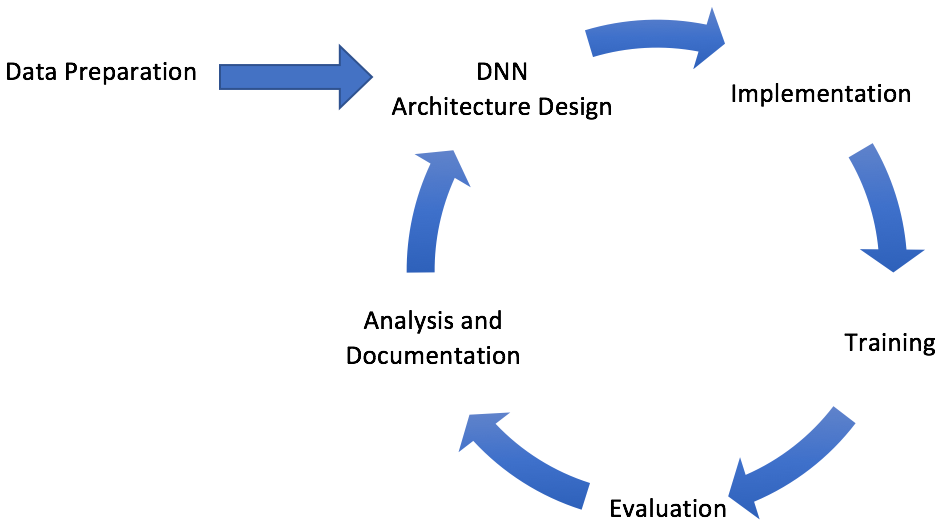
\includegraphics[scale=0.3]{Workflow}
    \caption{Project Workflow}
    \label{fig:workflow}
\end{figure}

\subsection{Risk Assessment}

After literature review, an assessment of the risks associated with this project was carried out. Consequently, difficulty in reproducing the results of the previous research, was identified as one of the main risks in this project. Therefore, it was decided that in case of facing such problem, instead of reproducing the results, the reported results would be used as a basis for comparing the outcome of this project with the state of the art.  
